\documentclass[11pt,a4paper]{article}
\usepackage[utf8]{inputenc}
\usepackage[german]{babel}
\usepackage[T1]{fontenc}
\usepackage{amsmath}
\usepackage{amsfonts}
\usepackage{amssymb}
\usepackage{graphicx}
\usepackage{listings}
\usepackage[left=2.5cm,right=2.5cm,top=2.5cm,bottom=2cm]{geometry} 
\usepackage{tabularx}
\usepackage{blindtext}
\usepackage{hyphenat}
\usepackage{hyperref}
\usepackage{nameref}
\usepackage{float}
\usepackage{pgfplots}
\usepackage{tikz}
\usepackage{caption}
\usepackage{float}
\usepackage{newclude}
\DeclareUnicodeCharacter{00B0}{~}

\makeatletter
\makeatother

\newcommand{\ms}{\mathrm{ms}}

\newcommand{\bibLabel}[1]{\label{#1}\hypertarget{#1}{}}
\newcommand{\bibRef}[1]{\hyperlink{#1}{$^{[\ref*{#1}{}]}$}}

\newcommand{\productName}{VARROAZERSTÖRER 3000}
\begin{document}

\begin{center}
\Large{Spezialschulteil des Albert-Schweitzer-Gymnasiums Erfurt}\\[1.5ex]
\large{Seminarfacharbeit Klasse 11/12}
\end{center}
\normalsize


\thispagestyle{empty}
\vspace*{2cm} % Vertikaler Abstand
\begin{center}

\includegraphics[scale=.4]{images/logo}\\
\vspace*{2cm}
% Titel der Arbeit:
\Huge{\textbf{Entwicklung des \\VARRODETEKTORS 187}} 

\end{center}
\normalsize

\vspace*{4cm}
\Large{ % Große Schriftgröße
\begin{tabular}{ll}
Fachbetreuer: & Herr Süpke \\
Seminarfachbetreuer: & Frau Nadler \\

Name: & Albert H. Dehne \\
& Daniel F. Cermann\\
& Richard Ueltzen\\

Datum: & \today
\end{tabular}
}
\normalsize % Setzt zurück auf normale Schriftgröße

\newpage

% Inhaltsverzeichnis
\thispagestyle{empty}
\setcounter{page}{1}
\tableofcontents
\newpage


% ---------------------------------------
% ------------Einleitung-----------------       1 Seite
% ---------------------------------------
\section{Einleitung}
Jährlich sterben etwa 15\% der Bienenvölker in Deutschland an den Folgen von Varroamilbenbefall(i1).
Viele weitere Bienenstöcke werden zusätzlich durch den Parasiten stark geschwächt.\\
Dies ist ein großes Problem: Nicht nur für Bienen, sondern auch für Natur und Mensch. Weltweit sind 80\% der Pflanzen auf die Bestäubung von Bienen angewiesen. Die enorme Bedeutung der Bienen spiegelt sich auch im geschätzten Wirtschaftswert der Biene, etwa 265 Milliarden Euro jährlich, wieder(i2).
Aktuell gibt es verschiedene Wege die Varroamilbe zu bekämpfen. Jedoch sind die meisten dieser Methoden ineffizient \footnote{starke Quelle}. Des Weiteren sind die ökologischen Schäden, welche die Anwendung der gängigen Säurebehandlung hinter sich ziehen, nicht zuvernachlässigen. Sie sollten mit dem Nutzen in jedem Falle abgewogen werden. Andere Bekämpfungsmethoden sind unter anderem die Wärmebehandlung von ganzen Bienenstöcken. Diese hat jedoch nur einen Wirkungsgrad von circa 60\%.\\
Wir haben uns zum Ziel gesetzt, eine neue Behandlungsmethode zu entwickeln. Dabei ist uns besonders wichtig, den ökologischen Schaden für die Bienen und die Umwelt so gering wie möglich zu halten. Unser Ziel ist dabei, nur die betroffenen Bienen zu behandeln. Diese wollen wir durch eine optische Erkennung der Varroamilben am Bienenstockeingang ermöglichen. Anschließend sollen befallene Bienen erkannt und abgesondert werden. Nach diesem Prozess kann die betroffenen Biene behandelt werden und wieder in den Bienenstock zurückgeführt werden. Dieses Vorgehen ermöglicht darüberhinaus eine ganzjährige Behandlung eines Bienestocks und hat im hat im Gegensatz zu bisherigen Methoden das Potenzial, das Eindringen der Varroamilben in den Stock, präventiv zu verhindern.  Dem gegenüber steht z.B. die Säurebehandlung, welche nur durchgeführt werden kann, wenn die Bienen keinen Nektar sammeln. Unser Hauptziel besteht darin, den erstmaligen Befall mit der Varroamilbe zu verhindern. Eine Kombination von konventionellen Behandlungsmethoden und unserer neuen Mehthode könnte Bienenstöcke vollständig von Milbenbefall befreien.\\
In unserer Arbeit fokussieren wir uns auf die optische Varroamilbenerkennung, um die Grundlage zur Bekämpfung zu schaffen. Des Weiteren können durch die Erkennung des Schädlings Forschungsdaten zum Verhalten von Bienen und Varroamilben kostenkünstig erhoben werden. Die Bekämpfung der Varroamilben arbeiten wir konzeptionell aus und sammeln unsere technischen Umsetzungsideen.\\
An dieser Stelle möchten wir ein Dankeschön für die Unterstützung an unseren Fachbetreuer Johannes Süpke und unsere Seminarfachbetreuerin Dörte Nadler aussprechen. Des Weiteren möchten wir uns in besonderer Weise für die tatkräfte Unterstützung unseres Außenbetreuers Jan Rimbach bedanken, welcher uns stets mir fachkundiger Auskunft zur Seite stand und uns mit der aktuellen Technik ausgestattet hat. Ein weiterer Dank geht an das Schülerforschungszentrum, vertreten durch Frank Paulig. \\




% ---------------------------------------
% ----------Theoriekapitel---------------           2 - 3 Seiten ~ Albert
% ---------------------------------------
\newpage
\section{Verhalten von Bienen und Varroamilben}
\begin{itemize}
	\item aktuelle Bekämpfungsmöglichkeiten
	\item was sind Bienen?
	\item Aufbau/Physiologie von Bienen
	\item Was sind Varroen?
	\item Aufbau von Milben/Wo sitzen die Milben?/Eigenschaften, die wir uns für die Erkennung zu nutze machen können?
\end{itemize}

% ---------------------------------------
% ----------Vorbetrachtungen-------------           2 - 3 Seiten ~ Daniel
% ---------------------------------------
\newpage
\section{Vorbetrachtungen und Experimente} \label{section:Vorbetrachtungen}

% $\rightarrow$ mögliche Lösungsansätze\\
% $\rightarrow$ Mit Experimenten flexen\\

\subsection{Aufbaumöglichkeiten der Varroaerkennung}
Bevor wir mit dem Bau von Prototypen begannen, haben wir durch Brainstorming so viele Ideen wie möglich gesammelt.\\
Ein erster Ansatz war, die Bienen mit Kameras zu filmen und somit die Milben optisch zu erkennen. Durch Anpassung der äußeren Bedingungen, wie Lichtverhältnisse, wollten wir die Erkennung so zuverlässig wie möglich gestalten.\\
Eine weitere Idee beruht auf einer möglichen Wärmedifferenz zwischen Bienen und Milben: Wäre die Differenz der Körpertemperaturen nicht marginal, könnten wir beim Filmen mit Wärmebildkameras vermutlich Milben als warme bzw. kalte Punkte auf den Bienen erkennen. Diese Methode hätte allerdings beträchtliche Nachteile: Zum einen sind Infrarot-Kameras mit der von uns benötigten Auflösung sehr teuer. Unsere Varroamilbenerkennung würde also auch langfristig nicht preiswert sein und somit keine weitreichende Anwendung finden. Außerdem sind Bienen wechselwarm \footnote{https://link.springer.com/article/10.1007/BF00298066}. Die stark von der Außentemperatur abhängenden Schwankungen der Körperkerntemperatur würden wahrscheinlich zu Ungenauigkeiten und ungeahnten Problem bei der Milbenerkennung führen.\\
Auch andere Möglichkeiten, die wir in Betracht zogen, hatten große Nachteile oder waren mit unseren Mitteln nicht umsetzbar. Also kamen wir zu dem Schluss, das Erkennen der Milben mit Kameras durchzuführen.\\
Nach unserer ersten Abwägung von Ideen war der nächste Schritt, das Scannen der Bienen konzeptionell zu planen. Alle unserer Überlegungen beruhten dabei auf einem von zwei grundsätzlichen Ansätzen: Entweder jede Biene wird durch Bewegung der Kamera bzw. Veränderung des Zooms einzeln fokussiert und anschließend auf Varroen gescannt oder eine Kamera ist statisch und überwacht gleichzeitig mehrere Bienen aus ihrem Sichtfeld. Eine konzeptionelle Gegenüberstellungen der beiden Möglichkeiten ist in Abbildung ? (Anhang Seite ?) zu erkennen. Bei der Entscheidung für eine Herangehensweise, mussten wir Klarheit und Auflösung der Bilder gegen Kosten und Aufwand abwägen.\\
Der erste der beiden Ansätze hatte den großen Vorteil, dass die Auflösung der fotografierten Biene höher wäre. Versuche von uns haben gezeigt, dass ein kleinerer Abstand der Kamera zur Biene für die Bildqualität und somit auch für die Varroaerkennung, unabhängig von der verbesserten Auflösung, förderlich ist. Allerdings brächte man für eine Durchführung dieser Idee in jedem Fall mechanische Vorrichtungen. Die Skizze einer möglichen Umsetzung mit auf linearen Achsen montierten Spiegeln ist im Anhang auf Seite ???? zu erkennen.\\
Neben den theoretischen Überlegungen führten wir außerdem Tests mit Servomotoren durch. In einem einfachen, 3D-gedruckten Versuchsaufbau testeten wir wie schnell die Kamera auf beliebige Stellen des Flugbretts geschwenkt werden kann (siehe Anhang S. ???). Die Versuche ergaben, dass wir pro Sekunde etwa eine Biene untersuchen könnten. Natürlich ließe sich diese Rate verbessern. Angesichts der Anforderung im Sommer bis zu als 20 Bienen pro Sekunde erkennen zu können, häuften sich die Argumente trotz dessen gegen diese Idee. Bei Abschätzungen der Kosten, Geschwindigkeitslimitierenden Faktoren, Lautstärke und Wartungsaufwand des Systems entschieden wir uns schließlich ganz gegen diesen Ansatz.\\
Das zweite Konzept ist in der Umsetzung rein vom Versuchsaufbau um einiges leichter. Trotzdem mussten wir vor der Umsetzung einige Optionen abwägen. Beispielsweise mussten uns entscheiden, ob viele billige Kameras, die jeweils nur einen kleinen Bereich des Flugbretts überwachen oder wenige Kameras mit einer sehr hohen Bildqualität und Auflösung bessere Resultate erzielen würden. Wir entschieden uns für die zweite Option. Unsere Überlegungen dazu sind im Anhang auf Seite ??? nachzuvollziehen.
Eine weitere, besonders schwierige Frage, die sich uns stellte, war, ob wir auch die Unterseite der Bienen durch Kameras untersuchen sollten. Aufgrund des ungemein größeren Aufwands und der Tatsache, dass Milben hauptsächlich auf dem Rücken der Bienen sitzen haben wir uns dagegen entschieden.\\

\subsection{Experimente zur Optimierung der Fotoqualität}
Um Varroamilben möglichst zuverlässig auf Bienen zu erkennen, muss der Kontrast zwischen Milbe und Biene so ausgeprägt wie möglich sein. Durch Durchführung systematischer Experimente haben wir die Rahmenbedingungen für ein solches Optimum so präzise wie möglich Festgestellt.\\
Bei allen durchgeführten Versuchen fotografierten wir tote Bienen, auf deren Rücken oder Panzer eine Varroamilben saß. Dabei haben wir von außen kommendes Licht fast vollständig abgeschirmt, um zufällige Fehler durch Sonnenlicht oder andere Beleuchtungsänderungen zu vermeiden. Somit hatten wir die Möglichkeit alle Bedingungen eines Fotos konstant zu halten und nur eine der Faktoren sehr gezielt zu verändern.\\
Bei unseren Untersuchten beschränkten wir uns speziell auf die optimale Helligkeit und Wellenlänge der Belichtung, sowie die beste Beschaffenheit und Farbe des Untergrunds.\\
Die Ergebnisse unserer Versuche bezüglich der optimalen Wellenlänge der Beleuchtung waren eindeutig. Die Milben sind bei Licht mit einer besonders hohen Wellenlänge am besten zu erkennen (siehe Anhang S. ???). Die Wellenlänge sollte zwischen 900 nm und 950 nm liegen. das entspricht kurzwelligem Infrarotlicht\footnote{\url{https://www.heizstrahler-direkt.de/blog/ir-heizstrahler-die-drei-verschiedenen-strahlungstypen/}}.\\
Höher sollte die Wellenlänge der Beleuchtung nicht sein. Denn gängige Fotosensoren, Objektive und Linsen sind für sichtbares Licht optimiert. Außerhalb eines Toleranzbereiches bräuchten wir spezielle, teure Optik.\\
Infrarotes Licht wird zudem von Bienen nicht gesehen. Bienen nehmen nämlich Licht nur bis zu einer Wellenlänge von etwa 650nm wahr\footnote{\url{https://honeybeehq.com/how-do-bees-see-the-world-this-is-their-superpower/}}. Im Anhang auf S. ??? ist das für Bienen sichtbare Spektrum zu sehen. Eine Beleuchtung mit Infrarotem Licht können wir also benutzen, ohne die Bienen einzuschränken.\\
Bei den Experimenten zum Untergrund ergab sich, dass jegliche Reflexionen und Streuungen des Lichts den Kontrast zwischen Milbe und Biene verschlechtert. Der beste Untergrund sollte somit schwarz sein und möglichst wenig reflektieren.


% ---------------------------------------
% --------------Prototype----------------           3 Seiten ~ Daniel
% ---------------------------------------
\newpage
\section{Entwicklung und Verbesserung verschiedener Prototypen}
\subsection{Angewandte Arbeitsmethoden}
Die wohl wichtigste von uns angewandte Arbeitsmethode ist das Prototyping. Prototyping ist ein Verfahren zum Austesten von angestrebten Ergebnissen mittels aufwandsarmer, günstiger Testversionen\footnote{https://www.businessinsider.de/gruenderszene/lexikon/begriffe/prototyping/}. Es wird sich schrittweise, durch ständige Ausbesserung von Fehlern oder Lücken, einer möglichst optimalen Lösung angenähert. Unwichtige Details und ablenkende, kleinere Probleme können bei diesem Prozess vorerst ignoriert werden. Der Fokus auf die wesentlichen Herausforderung kann somit erhalten bleiben.\\
Dieses Verfahren ist in unserem Projekt besonders nützlich, da bei der Arbeit mit Bienen viele Fehlerquellen sehr schwer vorhersehbar sind. Wir wussten zu Beginn unserer Arbeiten nicht, wie genau ein mögliches Endprodukt aussehen könnte. Durch das Herstellen von Prototypen konnten wir auch alle unsere Lösungsansätze wenigstens grundätzlich testen. So konnten wir sehr viele vage Ideen testen und immer weiter konkretisieren.\\
Für diese Arbeitsweise war das Arbeiten mit den uns zur Verfügung stehenden 3D-Druckern sehr wichtig. Die Kombination aus Druckern und einem CAD-Programm ermöglicht sehr schnelle Umsetzung von Ideen. CAD kommt aus dem Englischen und steht für ,,Computer-Aided Design''. 
\begin{itemize}
    \item Rapid Prototyping
    \item -> CAD-Programm: Fusion 360; um Maße richtig zu treffen: mehrere Versuche
    \item Prototypen schnell und leicht an Bienen anbringbar -> schnelles Feedback
    \item Schreiben der Software und Machen von Fotos bzw. Starten von Videos remote möglich -> Linux command line Wissen
	\item Prototypen
	\item 3D-Drucken und Designen
	\item schnell an Bienen anbringen
	\item Linux-command-line Wissen genutzt
\end{itemize}
\subsection{Technische Grundlagen}
Bevor wir überhaupt die Möglichkeit hatten, Prototypen zu bauen und zu testen, mussten einige Grundgegeben sichergestellt werden.\\
Zum einen brauchten wir eine stabile Stromquelle für Langzeittests. Denn bei den uns zur Verfügung stehenden Bienenkästen ist keine Stromversorgung durch das Stromnetz möglich. Als Energiespeicher brauchten benutzen wir eine alte Autobatterie. Mit einer Spannung von 12V und einer Kapazität von etwa 50 Amperestunden sollte diese bei einem Verbrauch von höchstens 15W länger als 40 Stunden halten. Die Batterie wir durch eine 20W Solarzelle aufgeladen. Außerdem wird die 12 Volt Ausgangsspannung der Batterie durch einen Spannungswandler auf die für von Einplatinencomputer gängige Spannunng 5 Volt heruntergewandelt. Der gesamte Aufbau der Stromversorgung ist im Anhang auf Seite ??? zu erkennen.\\
Außerdem mussten wir für leichten und schnellen Zugriff auf den \productName \ haben eine WLAN-Verbindung im Garten herstellen. Besonders für den Entwicklungsprozess ist das wichtig.

\begin{itemize}
	\item Stromversorgung sichern
	\item WLAN-Verbindung
	\item technische Entscheidungen: erst Raspberry Pi, dann Jetson Nano (ist cool und schnell)
\end{itemize}

\subsection{Erster Prototypen}
Bereits im Herbst 2020 haben wir mit dem Bau erster Prototypen begonnen. Diese waren nicht besonders funktional. Die einzige Funktion war es, erste Fehlerquellen ausfündig zu machen. Wären die Bienen beispielsweise von der Technik oder dem Vorbau am Bienenstockeingang gestört worden, hätten wir diese grundsätzlichen Probleme bereits frühzeitig entdeckt.\\
Die in diesem Protoyp verbaute Rechentechnik ist ein Raspberry Pi, ein sehr beliebter Einplatinencomputer. Als Kamera haben wir das zugehörige Kameramodul ,,Raspberry Pi Camera V2'' verbaut. Diese hat eine Auflösung von 8 Megapixel, der Sensorbereich ist allerdings sehr klein, was sich negativ auf die Bildqualität auswirkt. Das Modul ist sehr beginnerfreundlich und ist vergleichsweise preiswert. Für erste Tests war dieses Modul also ausreichend, ließ allerdings noch Verbesserungsmöglichkeiten offen.



\subsection{Zweiter Protoyp}
\begin{itemize}
    \item groß -> überblickt gesamtes Flugbrett
    \item mit Technik, die wir langfristig nutzen wollen:
    \begin{itemize}
        \item Jetson Nano, 2 x ?MP MIPI Camera, 940nm Led-Strips
    \end{itemize}
    \item kurze Tests, mussten wir allerdings abbrechen (wegen einigen Fehlerquellen)
    \item Fehlerquellen
    \begin{enumerate}
        \item Bienen akzeptieren Flugbrett nicht
        \item Spiegelungen in Plexiglas, das Bienen von Kameras trennt
        \item super vieeel
    \end{enumerate}
\end{itemize}



\subsection{Dritter Protoyp}
\begin{itemize}
    \item Ausbesserungen der meisten Fehler
    \item ausgiebigere Tests; 40GB Video- und Bilddaten
\end{itemize}


% ---------------------------------------
% --------------Software-----------------           4 Seiten ~ Richard
% ---------------------------------------
\newpage
\section{Programmierung der Milbenerkennung} \label{section:Programmierung}
\subsection{Architektur der Milbenerkennung}
Die Eingabe für das Programm ist eine Video-Datei. Auf jedem Videoeinzelbild werden um alle Bienen unter Verwendung eines durch uns trainierten neuronalen Netzes zur Bienenerkennung so genannte \textit{Bounding Boxes} ermittelt. Dabei handelt es sich um das kleinste Rechteck mit horizontalen und vertikalen Seiten, welches die Biene vollständig enthält. Mit einem eigenen Algorithmus zur Videoverfolgung der Bienen kann das Programm einen zeitlichen Zusammenhang zwischen den analysierten Bildern herstellen. Das heißt, die Bewegung jeder Biene wird verfolgt, sodass das Programm erkennt, dass eine Biene die sich zwischen zwei Bildern bewegt, das selbe Objekt bleibt. In allen ermittelten Bounding Boxes wird geprüft, ob sie Varroen enthalten. Falls dem so ist, wird die entsprechende Biene als infiziert markiert. Die Biene behält diesen Status in allen weiteren Videoeinzelbildern, was durch die Videoverfolgung möglich ist. Das führt zu einer Minimierung der Fehler erster Art bei der Milbenerkennung, denn es ist ausreichend, dass die Milbe in einem Einzelbild erkennbar ist, aber die Biene wird in vielen Bildern untersucht, während sie den aufgenommenen Bereich durchquert.
\subsection{Erstellung eines Modells zur Bienenerkennung}
Für das Training des neuronalen Netzes zur Bienenerkennung haben wir eigene Trainingsdaten erstellt. Denn es gibt keine öffentlichen Daten zu diesem Problem im Internet, die unseren Anforderungen entsprechen. Dafür haben wir durch ein selbst geschriebenes Python-Skript \textit{extract\_images.py} aus 40-sekündigem Videomaterial jedes zehnte Videoeinzelbild gespeichert. Mit diesen 120 Bildern haben wir auf \textit{roboflow.com} einen eigenen Datensatz kuratiert, indem wir in jedem Bild manuell die Bounding Boxes aller Bienen eingezeichnet haben. Wegen unserer Methoden des Versuchs und Irrtums und des Literaturstudiums\bibRef{annotate-tips} konnten wir dafür Regeln definieren, mit denen wir einen hochwertigen Datensatz erstellen konnten. Bounding Boxes sollen
\definecolor{ora}{rgb}{1,0.5,0}
\definecolor{pur}{rgb}{1,0,1}
\definecolor{blu}{rgb}{0,1,1}
\begin{itemize}
    \item[\textcolor{ora}{\textbullet}] so klein wie möglich sein,
    \item[\textcolor{ora}{\textbullet}] aber den gesamten Kopf, Rumpf und Hinterteil der Biene enthalten,
    \item[\textcolor{ora}{\textbullet}] aber nicht die Flügel und Beine der Biene enthalten,
    \item[\textcolor{pur}{\textbullet}] und verdeckte Körperteile der Biene enthalten, als wären sie sichtbar,
    \item[\textcolor{blu}{\textbullet}] und auch für Bienen am Bildrand gezeichnet werden.
\end{itemize}
Abbildung \autoref{fig:annotated_edited} wurde unter diesen Regeln annotiert, wobei einige Bounding Boxes, weil sie eine der Regeln demonstrieren, in der entsprechenden Farbe umgefärbt wurden.
\begin{figure}[H]
    \centering
    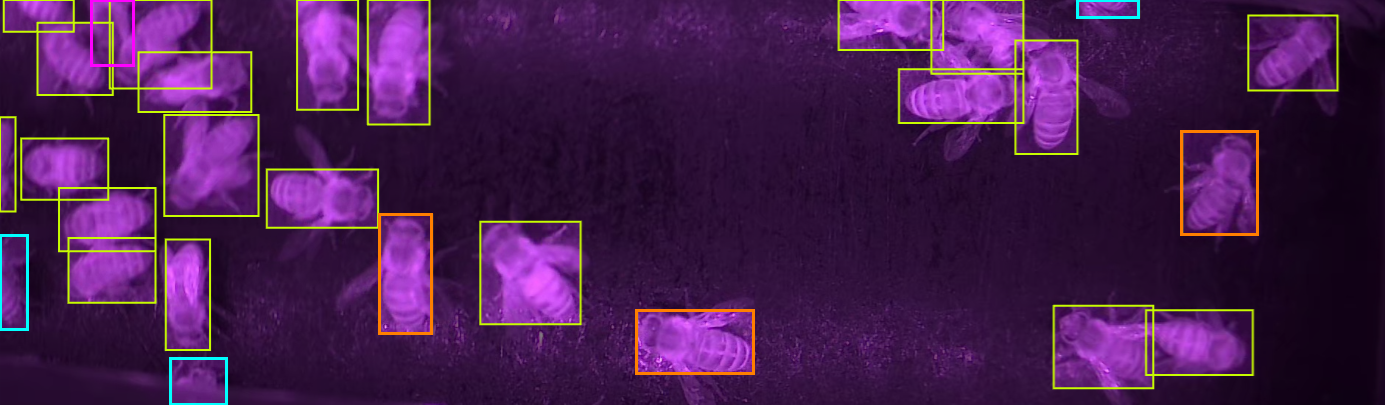
\includegraphics[width = .8\textwidth]{images/annotated_edited.png}
    \caption{Regelkonform annotiertes Bild}
    \label{fig:annotated_edited}
\end{figure}
\noindent
Nachdem alle Bilder mit Bounding Boxes versehen waren, haben wir außerdem die horizontale Spiegelung jeden Bildes zum Datensatz hinzugefügt. Durch diese so genannte \textit{Augmentation} haben wir mit einem geringem Aufwand die Größe des Datensatzes verdoppelt. Die Bounding Boxes haben wir im Darknet-Format exportiert. Dabei wird in einer Textdatei jedes Rechteck durch seine zwei x-Koordinaten und zwei y-Koordinaten gespeichert.\\
Wichtig ist für die Bienenerkennung eine Minimierung der Fehler auf fast null sowie eine sehr geringe Laufzeit, denn in jedem Videoeinzelbild werden alle Pixel untersucht. Deswegen haben wir als Modell zur Objekterkennung das neuronale Netz YOLOv4-tiny gewählt und uns für die YOLO-Implementierung in Darknet, einem Open-Source-Framework für neuronale Netze, entschieden. Es handelt sich dabei um eine verkleinerte Version des neuronalen Netzes YOLOv4. Das ist ein Modell, welches eine sehr hohe Leistungsfähigkeit, also geringe Fehlerzahl aufweist. Seine Besonderheit besteht darin, dass es die Bounding Boxes und die entsprechenden \textit{Scores}, das ist bei uns die Wahrscheinlichkeit, dass in der Box eine Biene ist, in einem Schritt anstatt nacheinander erstellt. Deswegen ist YOLOv4 ein \textit{one-stage detector} und es erhält daher seinen Namen \glqq You Only Look Once - version 4\grqq \, sowie seine hohe Effizienz.\\
YOLOv4-tiny verfügt über nur 29 \textit{convolutional layers} statt 53 und zwei \textit{YOLO layers} statt 3 im YOLOv4 Netzwerk\bibRef{darknet-yolov4}. Deshalb erreicht es eine noch geringere Laufzeit bei Erhaltung hoher Leistungsfähigkeit. Das verringerte auch die Trainingszeit des Modells um den gleichen Faktor. Deswegen konnten wir es auf Google-Colab, einem Cloud-Dienst, der für maximal zwölf Stunden kostenlos leistungsstarke GPU zur Verfügung stellt, vollständig trainieren.\\
\subsection{Implementierung der Videoverfolgung von Bienen}
Für jede Bounding Box von Bienen auf einem Videoeinzelbild wird ein dazugehöriges Bienen-Objekt, das in \textit{bee.py} definiert ist, erstellt. Dann wird nacheinander zu jedem Bienen-Objekt $b_0$ das Bienen-Objekt $b_1$ aus dem letzten Videoeinzelbild ermittelt, sodass der Abstand $d$ der Mittelpunkte von $b_0$ und $b_1$ am kleinsten ist. Wenn $d$ eine Grenze \textit{bee\_dist\_thresh}, die in \textit{settings.py} definiert ist, unterschreitet, nehmen wir an, dass $b_0$ die gleiche Biene wie $b_1$ ist. Deshalb erbt $b_0$ alle Eigenschaften von $b_1$ durch den Aufruf von $b_0.track(b_1)$, insbesondere ob sie infiziert ist. Außerdem löschen wir $b_1$ aus der Liste der Bienen aus dem letzten Videoeinzelbild, um Verdopplungen von Bienen zu verhindern. Wenn $d$ groß ist, dann ist $b_0$ zu keiner Biene aus dem vorherigen Videoeinzelbild nah. Das heißt, $b_0$ ist neu in das Bild gekommen oder hat sich sehr schnell bewegt. Zweiteres ist selten der Fall und führt deshalb zu einem kleinen Fehler.
\subsection{Erstellung eines Modells zur Varroaerkennung}
\subsection{Optimierung der Laufzeit}
Die Laufzeitoptimierung ist bei dem vorliegenden Problem von hoher Relevanz, da das Programm in Echtzeit laufen soll. Technologisch befinden wir uns gerade in der Übergangsphase, sodass Videoanalysen in Echtzeit auf kleinen Geräten schwierig aber möglich sind.\\
Wir haben alle rechenaufwändigen Operationen auf das Python-Modul für Computersicht \textit{cv2} (Computer Vision 2) ausgelagert. Diese behandelt ein Bild als \textit{numpy-array}, denn ein Bild ist eine Tabelle von RGB-Werten. Da \textit{numpy} in C++ implementiert ist, wird das Programm durch diese Auslagerung bis zu $100$ mal schneller. Für die optimale Ausnutzung dessen, haben wir an einen 14-stündigen \textit{cv2}-Kurs auf \url{udemy.com} teilgenommen\bibRef{udemy}.\\
Zur weiteren Verringerung der Laufzeit haben wir zunächst gemessen, welche Operationen einen großen Teil der Laufzeit verursachen. Dafür haben wir eine eigene, nutzerfreundliche \textit{Timer}-Klasse in \textit{timer.py} implementiert und verwendet. Damit haben wir schrittweise mit unserer Methode des Versuchs und Irrtums die Laufzeit weiter verringert.\\
Schon zu Anfang unserer Arbeit haben wir geplant, nur jedes $k$-te Videoeinzelbild zu analysieren. Aus unserem Literaturstudium ist allerdings hervorgegangen, dass alle modernen Videoformate zur Datenkompression die Änderungen zwischen aufeinanderfolgenden Videoeinzelbildern und nicht ganze Bilder speichern. Das ist eine Maßnahme zur so genannten Interframe-Kompression\bibRef{compression}. Für das Programm bedeutet das, dass man deutlich schneller das nächste Videoeinzelbild berechnen kann als zu einem Videoeinzelbild an einer bestimmten Stelle des Videos zu springen.\\
Deshalb haben wir mit unserer \textit{Timer}-Klasse einen eigenen Testaufbau erstellt, mit dem wir verschiedene Laufzeiten berechnen konnten.\\
Wir haben ermittelt, wie sich die Laufzeit $t_{iter}$ pro untersuchtem Bild und die Laufzeit $t_{real}$ pro Videosekunde, in Abhängigkeit von $k$ ändern. Dabei haben wir die Methoden $M1$, bei der man direkt zum $k-1$-nächsten Videoeinzelbild springt und dann das nächste Videoeinzelbild analysiert sowie die Methode $M2$, bei der man mehrfach das nächste Videoeinzelbild aufruft und bei jedem $k$-ten Aufruf das Bild analysiert, verglichen.
Dafür haben wir auf dem gleichen Gerät diese Werte ermittelt:
\begin{figure}[htb!]
    \centering
    \begin{tabular}{p{.07\linewidth}|p{.07\linewidth}|p{.5\linewidth}}
        Name & Wert & Definition \\ \hline
        $t_j$ & $44,7 \ms$ & Zeit zum Springen zu einem Videoeinzelbild \\ \hline
        $t_s$ & $5,4 \ms$ & Zeit zum Springen zum nächsten Videoeinzelbild \\ \hline
        $t_a$ & $29,2 \ms$ & Zeit zum Einlesen und Analysieren des nächsten Videoeinzelbilds
    \end{tabular}
\end{figure}\\
Für die Methoden $M1$ und $M2$ kann man die Laufzeiten so berechnen:
\begin{figure}[htb!]
    \centering
    \begin{tabular}{p{.07\linewidth}|p{.2\linewidth}|p{.2\linewidth}|p{.2\linewidth}|p{.2\linewidth}}
        $n$ & $t_{iter, M1}(k)$ & $t_{real, M1}(k)$ & $t_{iter, M2}(k)$ & $t_{real, M2}(k)$\\ \hline
        $1$ & $t_a + t_j$ & $(t_a + t_j) \cdot 30$ & $t_a$ & $t_a \cdot 30$\\
        $2$ & $t_a + t_j$ & $(t_a + t_j) \cdot 30 / 2$ & $t_a + t_s$ & $(t_a+t_s) \cdot 30 / 2$\\
        $3$ & $t_a + t_j$ & $(t_a + t_j) \cdot 30 / 3$ & $t_a + 2t_s$ & $(t_a+2t_s) \cdot 30 / 3$\\
        $\vdots$ & $\vdots$ & $\vdots$ & $\vdots$ & $\vdots$\\
        $x$ & $t_a + t_j$ & $(t_a + t_j) \cdot 30 / x$ & $t_a + (x-1)t_s$ & $(t_a+(x-1)t_s) \cdot 30 / x$
    \end{tabular}
\end{figure}\\
Damit können wir Graphen für die Laufzeiten der Algorithmen erstellen.
\begin{figure}[H]
    \centering
    \begin{minipage}{.45\textwidth}
        \begin{tikzpicture}[scale = .8]
            \begin{axis}[
                ymin = 0,
                ymax = 2.75,
                axis lines = left,
                xlabel = \(x\),
                ylabel = {$t_{real}(x) / \mathrm{s}$},
            ]
            \addplot [
                domain=1:12,
                samples=100, 
                color=blue,
                ]
                {0.03*(29.2 + 44.7)/x};
            \addlegendentry{$t_{real, M1}(x)$}
            \addplot [
                domain=1:12, 
                samples=100, 
                color=red,
            ]
            {0.03*(29.2 + 5.4*(x-1))/x};
            \addlegendentry{$t_{real, M2}(x)$}
            \end{axis}
        \end{tikzpicture}
        \caption{$M1-M2$-Vergleich}
        \label{fig:m1-m2}
    \end{minipage}
    \begin{minipage}{.45\textwidth}
        \begin{tikzpicture}[scale = .8]
            \begin{axis}[
                ymin = 0,
                ymax = 1.1,
                axis lines = left,
                xlabel = \(x\),
                ylabel = {$t_{real}(x) / \mathrm{s}$},
            ]
            \addplot [
                domain=1:5, 
                samples=100, 
                color=red,
            ]
            {0.03*(29.2 + 5.4*(x-1))/x};
            \addlegendentry{$t_{real, M2}(x)$}
            
            \end{axis}
        \end{tikzpicture}
        \caption{$M2$-Bewertung}
        \label{fig:m2}
    \end{minipage}
\end{figure}
\noindent
$k > 5$ würde zu einer zu geringen zeitlichen Auflösung führen, um die Erkennung aller Milben zu gewährleisten. Weil Abbildung \autoref{fig:m1-m2} zeigt, dass die Methode $M2$ für kleine $k$ deutlich schneller ist, haben wir uns deshalb für die Implementierung der Methode $M2$ entschieden.\\
Aus Abbildung \autoref{fig:m2} geht darüber hinaus hervor, dass ab $k = 3$ eine weitere Erhöhung von $k$ zu keiner starken Senkung der Laufzeit von $M2$ führt, weshalb $k \in \{1, 2, 3\}$ eine sinnvolle Wahl ist. Unter diesen drei Werten kann $k$ je nach Rechenleistung des Computers angepasst werden.

% ---------------------------------------
% ------Fortsetzungsmöglichkeiten--------       1 - 2 Seiten ~ Albert
% ---------------------------------------
\newpage
\section{Fortsetzungsmöglichkeiten}


% ---------------------------------------
% -------------Auswertung----------------           1 Seite ~ Alle
% ---------------------------------------
\newpage
\section{Auswertung}

% ---------------------------------------
% ---------------Anhang------------------
% ---------------------------------------
\newpage
\section{Anhang}
\subsection{Zu Kapitel \autoref{section:Vorbetrachtungen}}
\begin{figure}[H]
    \centering
    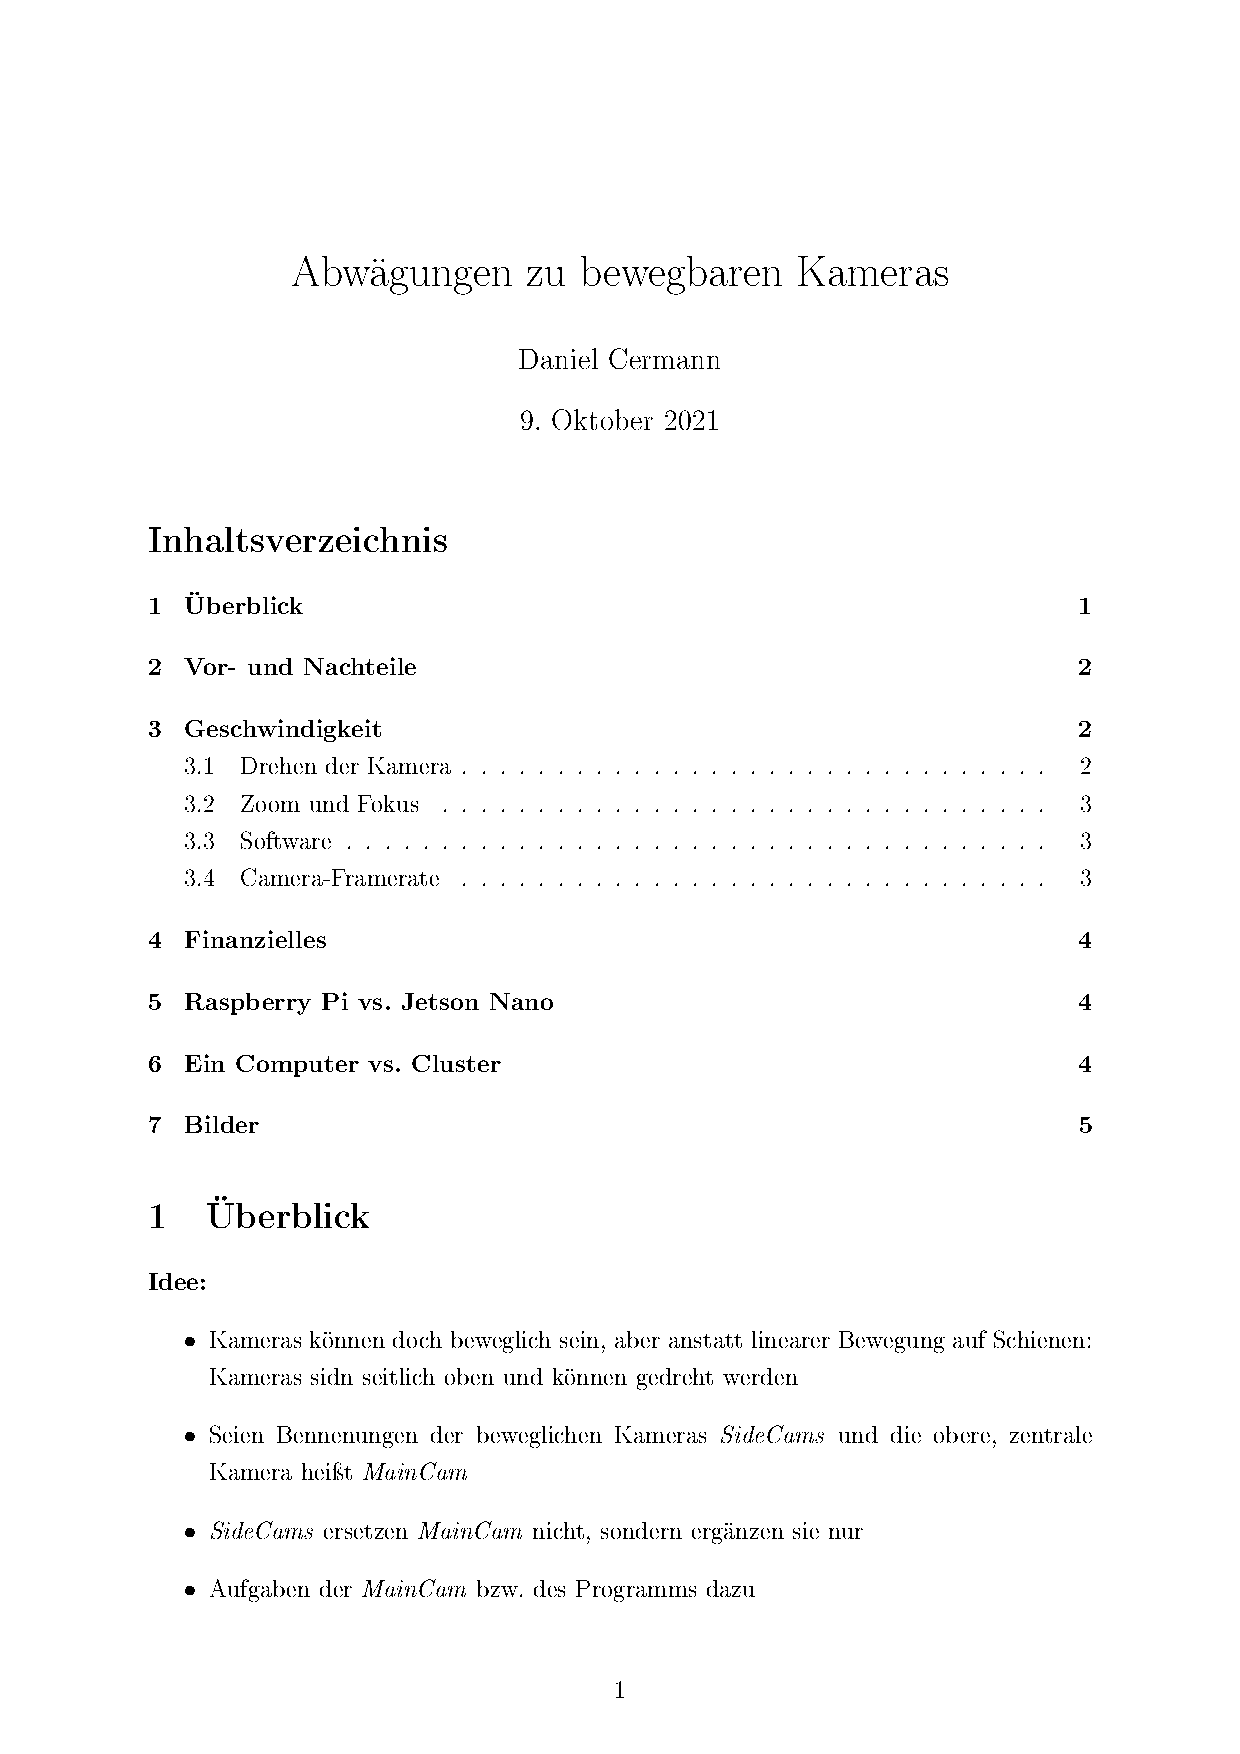
\includegraphics[page=1, scale=.3]{images/TPZ_Cameras_Idea.pdf}
    \includegraphics[page=2, scale=.3]{images/TPZ_Cameras_Idea.pdf}    
    \caption{Unsere Abwägungen zu bewegbaren Kameras}
    \label{fig:moving_cameras_considerations}
\end{figure}

\subsection{Zu Kapitel \autoref{section:Programmierung}}
\begin{figure}[!htb] \label{annotated1}
    \centering
	    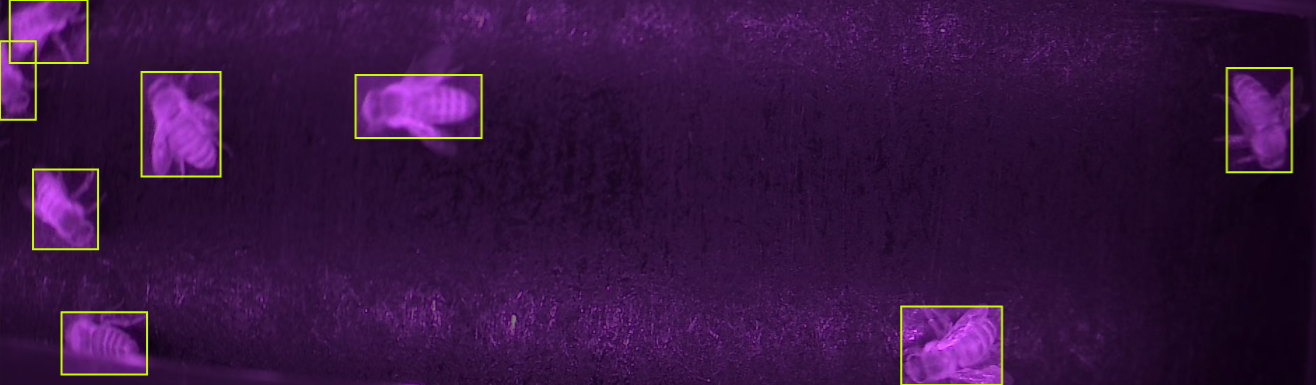
\includegraphics[width = .8\textwidth]{images/annotated1.png}
        \caption{Regelkonform annotiertes Bild}
\end{figure}

\begin{figure}[!htb] \label{annotated2}
    \centering
	    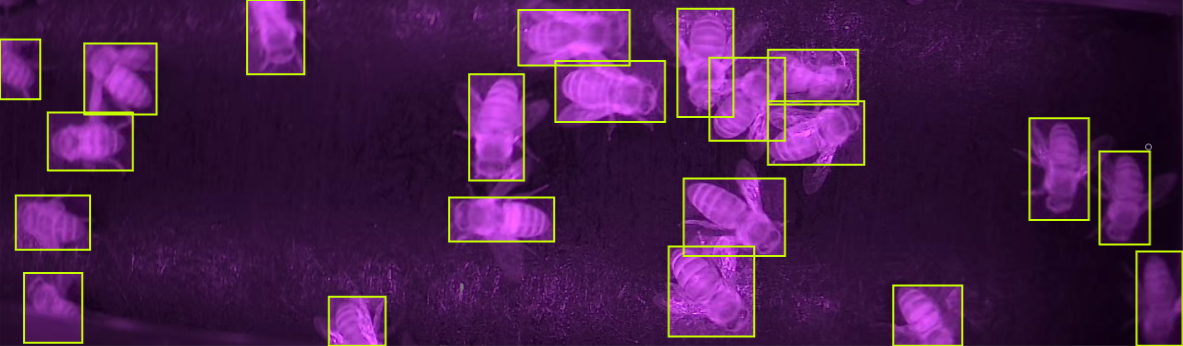
\includegraphics[width = .8\textwidth]{images/annotated2.png}
        \caption{Regelkonform annotiertes Bild}
\end{figure}

\begin{figure}[!htb] \label{annotated3}
    \centering
	    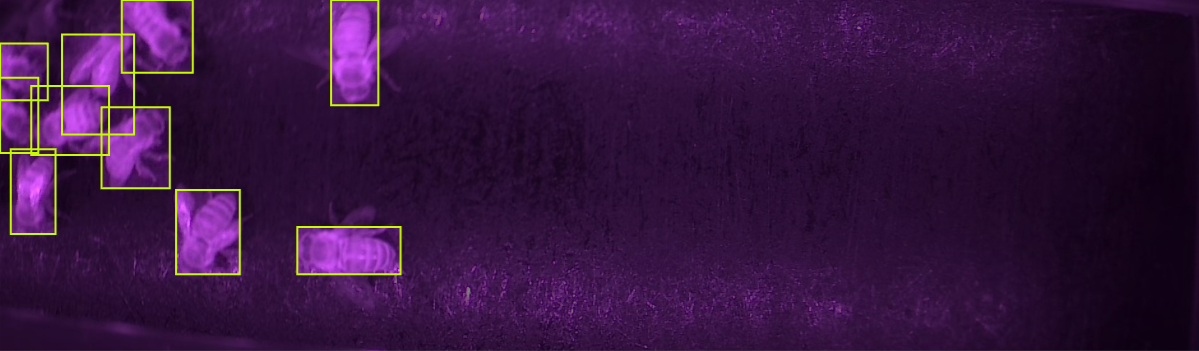
\includegraphics[width = .8\textwidth]{images/annotated3.png}
        \caption{Regelkonform annotiertes Bild}
\end{figure}
% ---------------------------------------
% --------Quellenverzeichnis-------------
% ---------------------------------------
\newpage
\section{Literatur- und Quellenverzeichnis}
\begin{thebibliography}
\\
\subsection{Gedruckte Literatur}

\subsection{Internetliteratur}
\setcounter{enumiv}{0}

\bibitem{br.de}\label{i1}
	\textsc{Autor unbekannt};
	\textit{Die Varroamilbe: Der gefährlichste Feind der Biene}\\
	\url{https://www.br.de/wissen/bienen-varroamilbe-bienensterben-lithiumchlorid-100.html}\\
	letzter Zugriff: 11.10.2021

\bibitem{bee-careful.com}\label{i2}
	\textsc{Autor unbekannt};
	\textit{Warum sind Bienen so wichtig?}\\
	\url{https://www.bee-careful.com/de/initiative/warum-sind-bienen-so-wichtig/}\\
	letzter Zugriff: 11.10.2021

\bibitem{blog.roboflow.com} \bibLabel{annotate-tips}
	\textsc{Nelson, Joseph};
	\textit{Seven Tips for Labeling Images for Computer Vision}\\
	\url{https://blog.roboflow.com/tips-for-how-to-label-images/}\\
	letzter Zugriff: 25.6.2021

\bibitem{darknet.com} \bibLabel{darknet-yolov4}
	\textsc{Alexey Bochkovskiy};
	\textit{Darknet releases}\\
	\url{https://github.com/AlexeyAB/darknet/releases}\\
	letzter Zugriff: 25.6.2021

\bibitem{udemy.com} \bibLabel{udemy}
	\textsc{Portilla, Jose};
	\textit{Python for Computer Vision with OpenCV and Deep Learning}\\
	\url{https://www.udemy.com/course/python-for-computer-vision-with-opencv-and-deep-learning/}\\
	letzter Zugriff: 23.04.2021

\bibitem{kompendium.infotip.de} \bibLabel{compression}
	\textsc{Autor unbekannt};
	\textit{Videokompression Grundlagen}\\
	\url{https://kompendium.infotip.de/grundlagen_videokompression.html/}\\
	letzter Zugriff: 17.09.2021

\end{thebibliography}

\end{document}